%%%%%%%%%%%%%%%%%%%%%%%%%%%%%%%%%%%%%%%%%%%%%%%%%%%%%%%%%%%%%%%%%%%%%%
%%  disstemplate.tex, to be compiled with latex.		     %
%%  08 April 2002	Version 4				     %
%%%%%%%%%%%%%%%%%%%%%%%%%%%%%%%%%%%%%%%%%%%%%%%%%%%%%%%%%%%%%%%%%%%%%%
%%								     %
%%  Writing a Doctoral Dissertation with LaTeX at		     %
%%	the University of Texas at Austin			     %
%%								     %
%%  (Modify this ``template'' for your own dissertation.)	     %
%%								     %
%%%%%%%%%%%%%%%%%%%%%%%%%%%%%%%%%%%%%%%%%%%%%%%%%%%%%%%%%%%%%%%%%%%%%%


\documentclass[12pt]{report}	% The documentclass must be ``report''.

\usepackage{utdiss2}  		% Dissertation package style file.


%%%%%%%%%%%%%%%%%%%%%%%%%%%%%%%%%%%%%%%%%%%%%%%%%%%%%%%%%%%%%%%%%%%%%%
% Optional packages used for this sample dissertation. If you don't  %
% need a capability in your dissertation, feel free to comment out   %
% the package usage command.					     %
%%%%%%%%%%%%%%%%%%%%%%%%%%%%%%%%%%%%%%%%%%%%%%%%%%%%%%%%%%%%%%%%%%%%%%

\usepackage{amsmath,amsthm,amsfonts,amscd} 
				% Some packages to write mathematics.
\usepackage{eucal} 	 	% Euler fonts
\usepackage{verbatim}      	% Allows quoting source with commands.
\usepackage{makeidx}       	% Package to make an index.
\usepackage{url}		% Allows good typesetting of web URLs.
%\usepackage{draftcopy}		% Uncomment this line to have the
				% word, "DRAFT," as a background
				% "watermark" on all of the pages of
				% of your draft versions. When ready
				% to generate your final copy, re-comment
				% it out with a percent sign to remove
				% the word draft before you re-run
				% Makediss for the last time.
\usepackage{latexsym}
\usepackage{natbib}
\usepackage{graphicx}
\usepackage{caption}
\usepackage{subcaption}
\usepackage{listings}
\usepackage{algorithm}
\usepackage{algpseudocode}
\usepackage{amssymb} 
\usepackage{color}
\usepackage{multirow}

\graphicspath{{nips15/}{RLLiterature/}}

\author{Shun Zhang}

\address{500 S State St\\ Ann Arbor, MI 48109}  % Required

\title{Parameterized Modular Inverse Reinforcement Learning}
                                                    % Required

%%%%%%%%%%%%%%%%%%%%%%%%%%%%%%%%%%%%%%%%%%%%%%%%%%%%%%%%%%%%%%%%%%%%%%
% NOTICE: The total number of supervisors and other members %%%%%%%%%%
%%%%%%%%%%%%%%% MUST be seven (7) or less! If you put in more, %%%%%%%
%%%%%%%%%%%%%%% they are put on the page after the Committee %%%%%%%%%
%%%%%%%%%%%%%%% Certification of Approved Version page. %%%%%%%%%%%%%%
%%%%%%%%%%%%%%%%%%%%%%%%%%%%%%%%%%%%%%%%%%%%%%%%%%%%%%%%%%%%%%%%%%%%%%

%%%%%%%%%%%%%%%%%%%%%%%%%%%%%%%%%%%%%%%%%%%%%%%%%%%%%%%%%%%%%%%%%%%%%%
%
% Enter names of the supervisor and co-supervisor(s), if any,
% of your dissertation committee. Put one name per line with
% the name in square brackets. The name on the last line, however,
% must be in curly braces.
%
% If you have only one supervisor, the entry below will read:
%
%	\supervisor
%		{Supervisor's Name}
%
% NOTE: Maximum three supervisors. Minimum one supervisor.
% NOTE: The Office of Graduate Studies will accept only two supervisors!
% 
%
\supervisor
	{Prof. Dana Ballard}

%%%%%%%%%%%%%%%%%%%%%%%%%%%%%%%%%%%%%%%%%%%%%%%%%%%%%%%%%%%%%%%%%%%%%%
%
% Enter names of the other (non-supervisor) members(s) of your
% dissertation committee. Put one name per line with the name
% in square brackets. The name on the last line, however, must
% be in curly braces.
%
% NOTE: Maximum six other members. Minimum zero other members.
% NOTE: The Office of Graduate Studies may restrict you to a total
%	of six committee members.
%
%
\committeemembers
	{Prof. Peter Stone}

%%%%%%%%%%%%%%%%%%%%%%%%%%%%%%%%%%%%%%%%%%%%%%%%%%%%%%%%%%%%%%%%%%%%%%

\previousdegrees{B.S.}
     % The abbreviated form of your previous degree(s).
     % E.g., \previousdegrees{B.S., MBA}.
     %
     % The default value is `B.S., M.S.'

%\graduationmonth{...}      
     % Graduation month, either May, August, or December, in the form
     % as `\graduationmonth{May}'. Do not abbreviate.
     %
     % The default value (either May, August, or December) is guessed
     % according to the time of running LaTeX.

%\graduationyear{...}   
     % Graduation year, in the form as `\graduationyear{2001}'.
     % Use a 4 digit (not a 2 digit) number.
     %
     % The default value is guessed according to the time of 
     % running LaTeX.

%\typist{...}       
     % The name(s) of typist(s), put `the author' if you do it yourself.
     % E.g., `\typist{Maryann Hersey and the author}'.
     %
     % The default value is `the author'.


%%%%%%%%%%%%%%%%%%%%%%%%%%%%%%%%%%%%%%%%%%%%%%%%%%%%%%%%%%%%%%%%%%%%%%
% Commands for master's theses and reports.			     %
%%%%%%%%%%%%%%%%%%%%%%%%%%%%%%%%%%%%%%%%%%%%%%%%%%%%%%%%%%%%%%%%%%%%%%
%
% If the degree you're seeking is NOT Doctor of Philosophy, uncomment
% (remove the % in front of) the following two command lines (the ones
% that have the \ as their second character).
%
\degree{MASTER OF SCIENCE}
\degreeabbr{M.S.}

% Uncomment the line below that corresponds to the type of master's
% document you are writing.
%
%\masterreport
\masterthesis


%%%%%%%%%%%%%%%%%%%%%%%%%%%%%%%%%%%%%%%%%%%%%%%%%%%%%%%%%%%%%%%%%%%%%%
% Some optional commands to change the document's defaults.	     %
%%%%%%%%%%%%%%%%%%%%%%%%%%%%%%%%%%%%%%%%%%%%%%%%%%%%%%%%%%%%%%%%%%%%%%
%
%\singlespacing
%\oneandonehalfspacing

%\singlespacequote
\oneandonehalfspacequote

\topmargin 0.125in	% Adjust this value if the PostScript file output
			% of your dissertation has incorrect top and 
			% bottom margins. Print a copy of at least one
			% full page of your dissertation (not the first
			% page of a chapter) and measure the top and
			% bottom margins with a ruler. You must have
			% a top margin of 1.5" and a bottom margin of
			% at least 1.25". The page numbers must be at
			% least 1.00" from the bottom of the page.
			% If the margins are not correct, adjust this
			% value accordingly and re-compile and print again.
			%
			% The default value is 0.125"

		% If you want to adjust other margins, they are in the
		% utdiss2-nn.sty file near the top. If you are using
		% the shell script Makediss on a Unix/Linux system, make
		% your changes in the utdiss2-nn.sty file instead of
		% utdiss2.sty because Makediss will overwrite any changes
		% made to utdiss2.sty.

%%%%%%%%%%%%%%%%%%%%%%%%%%%%%%%%%%%%%%%%%%%%%%%%%%%%%%%%%%%%%%%%%%%%%%
% Some optional commands to be tested.				     %
%%%%%%%%%%%%%%%%%%%%%%%%%%%%%%%%%%%%%%%%%%%%%%%%%%%%%%%%%%%%%%%%%%%%%%

% If there are 10 or more sections, 10 or more subsections for a section,
% etc., you need to make an adjustment to the Table of Contents with the
% command \longtocentry.
%
%\longtocentry 



%%%%%%%%%%%%%%%%%%%%%%%%%%%%%%%%%%%%%%%%%%%%%%%%%%%%%%%%%%%%%%%%%%%%%%
%	Some math support.					     %
%%%%%%%%%%%%%%%%%%%%%%%%%%%%%%%%%%%%%%%%%%%%%%%%%%%%%%%%%%%%%%%%%%%%%%
%
%	Theorem environments (these need the amsthm package)
%
%% \theoremstyle{plain} %% This is the default

\newtheorem{thm}{Theorem}[section]
\newtheorem{cor}[thm]{Corollary}
\newtheorem{lem}[thm]{Lemma}
\newtheorem{prop}[thm]{Proposition}
\newtheorem{ax}{Axiom}

\theoremstyle{definition}
\newtheorem{defn}{Definition}[section]

\theoremstyle{remark}
\newtheorem{rem}{Remark}[section]
\newtheorem*{notation}{Notation}

%\numberwithin{equation}{section}


%%%%%%%%%%%%%%%%%%%%%%%%%%%%%%%%%%%%%%%%%%%%%%%%%%%%%%%%%%%%%%%%%%%%%%
%	Macros.							     %
%%%%%%%%%%%%%%%%%%%%%%%%%%%%%%%%%%%%%%%%%%%%%%%%%%%%%%%%%%%%%%%%%%%%%%
%
%	Here some macros that are needed in this document:

\renewcommand{\P}{\mathbb{P}}
\newcommand{\Cov}{\mathrm{Cov}}
\newcommand{\E}{\mathrm{E}}
\newcommand{\Var}{\mathrm{Var}}

\newcommand{\latexe}{{\LaTeX\kern.125em2%
                      \lower.5ex\hbox{$\varepsilon$}}}

\newcommand{\amslatex}{\AmS-\LaTeX{}}

\chardef\bslash=`\\	% \bslash makes a backslash (in tt fonts)
			%	p. 424, TeXbook

\newcommand{\cn}[1]{\texttt{\bslash #1}}

\makeatletter		% Starts section where @ is considered a letter
			% and thus may be used in commands.
\def\square{\RIfM@\bgroup\else$\bgroup\aftergroup$\fi
  \vcenter{\hrule\hbox{\vrule\@height.6em\kern.6em\vrule}%
                                              \hrule}\egroup}
\makeatother		% Ends sections where @ is considered a letter.
			% Now @ cannot be used in commands.

\makeindex    % Make the index

%%%%%%%%%%%%%%%%%%%%%%%%%%%%%%%%%%%%%%%%%%%%%%%%%%%%%%%%%%%%%%%%%%%%%%
%		The document starts here.			     %
%%%%%%%%%%%%%%%%%%%%%%%%%%%%%%%%%%%%%%%%%%%%%%%%%%%%%%%%%%%%%%%%%%%%%%

\begin{document}

\copyrightpage          % Produces the copyright page.


%
% NOTE: In a doctoral dissertation, the Committee Certification page
%		(with signatures) is BEFORE the Title page.
%	In a masters thesis or report, the Signature page
%		(with signatures) is AFTER the Title page.
%
%	If you are writing a masters thesis or report, you MUST REVERSE
%	the order of the \commcertpage and \titlepage commands below.
%
\commcertpage           % Produces the Committee Certification
			%   of Approved Version page (doctoral)
			%   or Signature page (masters).
			%		20 Mar 2002	cwm

\titlepage              % Produces the title page.



%%%%%%%%%%%%%%%%%%%%%%%%%%%%%%%%%%%%%%%%%%%%%%%%%%%%%%%%%%%%%%%%%%%%%%
% Dedication and/or epigraph are optional, but must occur here.      %
%%%%%%%%%%%%%%%%%%%%%%%%%%%%%%%%%%%%%%%%%%%%%%%%%%%%%%%%%%%%%%%%%%%%%%
%
\begin{acknowledgments}		% Optional
\index{Acknowledgments@\emph{Acknowledgments}}%
I would like to express my gratitude to Prof. Dana Ballard and Prof. Mary Hayhoe
for the useful comments, remarks and engagement through the process of this
master thesis. Furthermore I would like to thank Prof. Peter Stone for
introducing me to the topic of reinforcement learning, and reading this thesis
as a committee member.

I would like to thank Matthew Tong, who conducted the human experiments. The
human experiment section would not be possible without his work. I would
like to thank Embodied Cognition Lab, directed by Prof. Dana Ballard, for their
feedback on this work. I would especially thank Ruohan Zhang, who I work with on
this project and on a paper submission.
\end{acknowledgments}


% The abstract is required. Note the use of ``utabstract'' instead of
% ``abstract''! This was necessary to fix a page numbering problem.
% The abstract heading is generated automatically.
% Do NOT use \begin{abstract} ... \end{abstract}.
%
\utabstract
\index{Abstract}%
Reinforcement learning and inverse reinforcement learning can be used to model
and understand human behaviors. However, due to the curse of dimensionality,
their use as a model for human behavior has been limited. Inspired by observed
natural behaviors, one approach is to decompose complex tasks into independent
sub-tasks, or modules. Using this approach, we extended an earlier work on 
modular inverse reinforcement learning, and developed what we called
parameterized modular inverse reinforcement learning algorithm. We first
demonstrate the correctness and efficiency of our algorithm in a simulated
navigation task. We then show our algorithm able to estimate a reward function
and discount factor for real human navigation behaviors in a virtual
environment, and train an agent that imitates the behavior of human subjects.
\footnote{This is the extension of a nonarchived paper in RLDM 2015, and
overlaps largely with a recent submission co-authored with Ruohan Zhang (equal
contribution), Matthew Tong, Mary Hayhoe and Dana Ballard.}
\indent

\tableofcontents   % Table of Contents will be automatically
                   % generated and placed here.

\listoftables      % List of Tables and List of Figures will be placed
\listoffigures     % here, if applicable.



%%%%%%%%%%%%%%%%%%%%%%%%%%%%%%%%%%%%%%%%%%%%%%%%%%%%%%%%%%%%%%%%%%%%%%
% Actual text starts here.					     %
%%%%%%%%%%%%%%%%%%%%%%%%%%%%%%%%%%%%%%%%%%%%%%%%%%%%%%%%%%%%%%%%%%%%%%
%
% Including external files for each chapter makes this document simpler,
% makes each chapter simpler, and allows for generating test documents
% with as few as zero chapters (by commenting out the include statements).
% This allows quicker processing by the Makediss command file in case you
% are not working on a specific, long and slow to compile chapter. You
% can even change the chapter order by merely interchanging the order
% of the include statements (something I found helpful in my own
% dissertation).
%
\chapter{Introduction}
Reinforcement learning has shown advantages in learning with only the task
specifications and feedback signals. A learning agent can interact with the
task, observe a current state, and take an action to observe
transition to the next state and receive a reward signal. The underlying model is either
known or not by the agent. Concretely, the task is formulated as a
Markov Decision Process (MDP), which will be defined in details later.
The objective of the task is to take actions to maximize the accumulated payoff.
In recent years, reinforcement learning has been successfully applied to
helicopter control \cite{ng2006autonomous} and Atari games \cite{mnih2013playing}.

Reinforcement learning is analogous to the way that human learns. Human infants
have limited prior knowledge of the world. They can learn to optimize
their behavior by observing the environment and perceiving joy or pain. So it is
of interest to discover the underlying decision model of human. In both fields
of artificial intelligence and neuroscience, people believe that reinforcement
learning is the model that can explain humans' learning.

However, humans are able to learn and accomplish complex tasks more efficiently than
reinforcement learning agents. The possibilities are that humans have some prior
knowledge on how to accomplish smaller and easier tasks. When they tackle a
complex task, they only need to decide which basic skills they need to use, and
how to combine them. Taking driving for example, humans learning to drive don't
take it as a completely new task. Many of their preliminary skills can
contribute to this new task. It is a complex behavior but a combination of
object avoidance, object following, etc.

To understand how human subjects make decisions and to test our hypothesis, we
propose an novel inverse reinforcement learning approach in this thesis.
We first tested the correctness and efficiency of this approach in a toy domain,
and further collected humans' behavior in a navigation task. We used such method
to analyze how the behavior is generated.

This thesis is organized as follows. Chapter~\ref{chp:mirl} introduces the
preliminary concepts of reinforcement learning, inverse reinforcement learning,
modular reinforcement learning and describes the proposed algorithm.
Chapter~\ref{chp:lr} reviews the literature on task decomposition in
reinforcement learning. We report our experimental results in
Chapter~\ref{chp:eval} and conclude in Chapter~\ref{chp:conclude}.


\chapter{Modular Inverse Reinforcement Learning}
\label{chp:mirl}
\input{nips15/2-preliminaries}
\input{nips15/2-1-modularRL.tex}
\input{nips15/2-2-modularIRL.tex}

\chapter{Literature Review}
\label{chp:lr}
Markov Decision Process
MDP:
\begin{itemize}
\item State: $S$.
\item Action: $A$.
\item Transition: $P: S \times A \times S \rightarrow \mathcal{R}$.
\item Reward: $R: S \times A \times S \rightarrow \mathcal{R}$.
\end{itemize}



Abstraction on MDP
\begin{itemize}
  \item Aggregate states: feature extraction. 
  \item Aggregate actions: {\bf option}. 
  \item Decompose transition: factored MDP. 
  \item Decompose value (abstract MDP): {\bf HAM, hierarchical RL, modular RL}.
\end{itemize}



MDP with Option
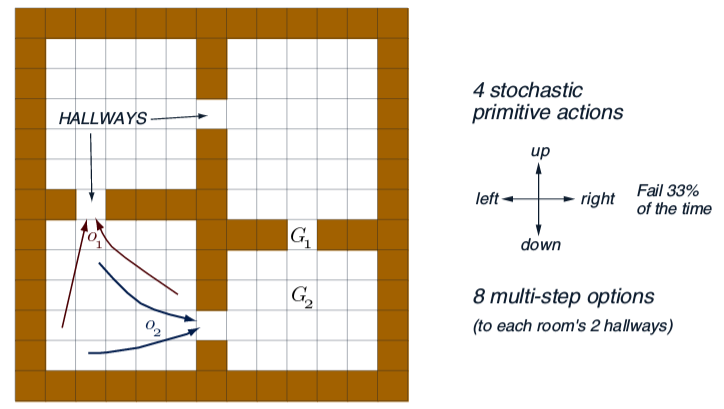
\includegraphics[width=0.8\columnwidth]{option.png}
\begin{itemize}
  \item Option: (start state, policy, termination condition).
\end{itemize}



\begin{itemize}
  \item State: $S$.
  \item Action: $A, {\color{red}O}$.
  \item Transition: $P: S \times {\color{red}\{A, O\}} \times S \rightarrow \mathcal{R}$.
  \item Reward: $R: S \times {\color{red}\{A, O\}} \times S \rightarrow \mathcal{R}$.
\end{itemize}



Hierarchies of Abstract Machines (HAM)
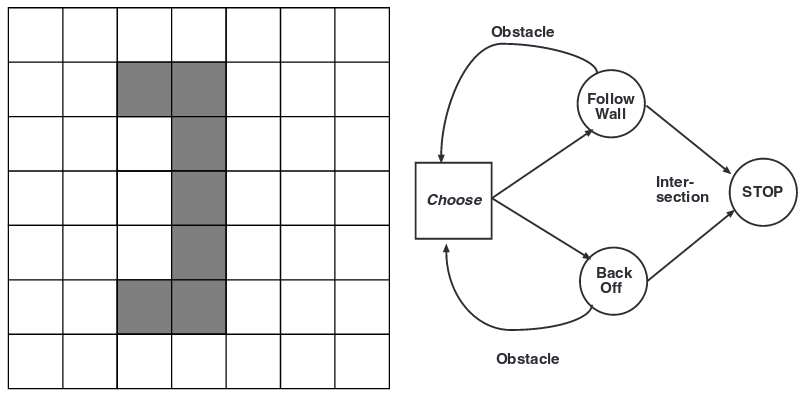
\includegraphics[width=0.8\columnwidth]{ham.png}
\begin{itemize}
  \item State machine of MDPs.
\end{itemize}



Hierarchical RL
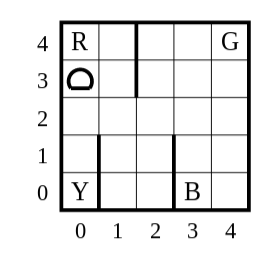
\includegraphics[width=0.4\columnwidth]{taxi.png}

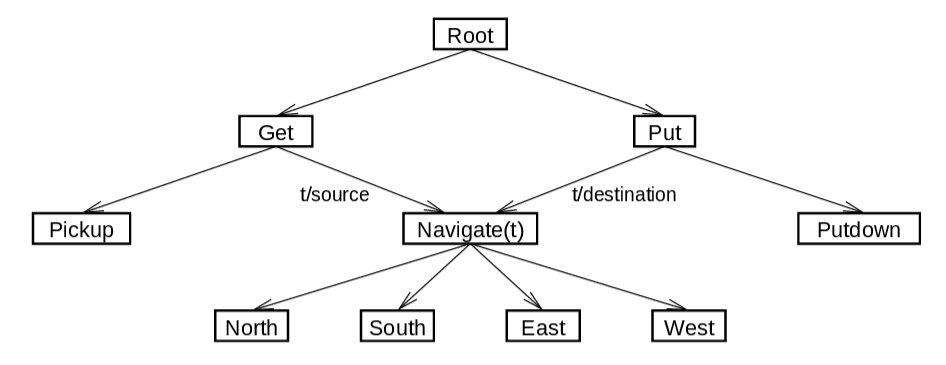
\includegraphics[width=0.8\columnwidth]{maxq.png}



Hierarchical RL
MDP:
\begin{itemize}
  \item State: {\color{red}$\mathcal{S}$}.
  \item Action: {\color{red}$\mathcal{A}$}.
  \item Transition: {\color{red}$\mathcal{T}$}.
  \item Reward: {\color{red}$\mathcal{R}$}.
\end{itemize}



Modular RL
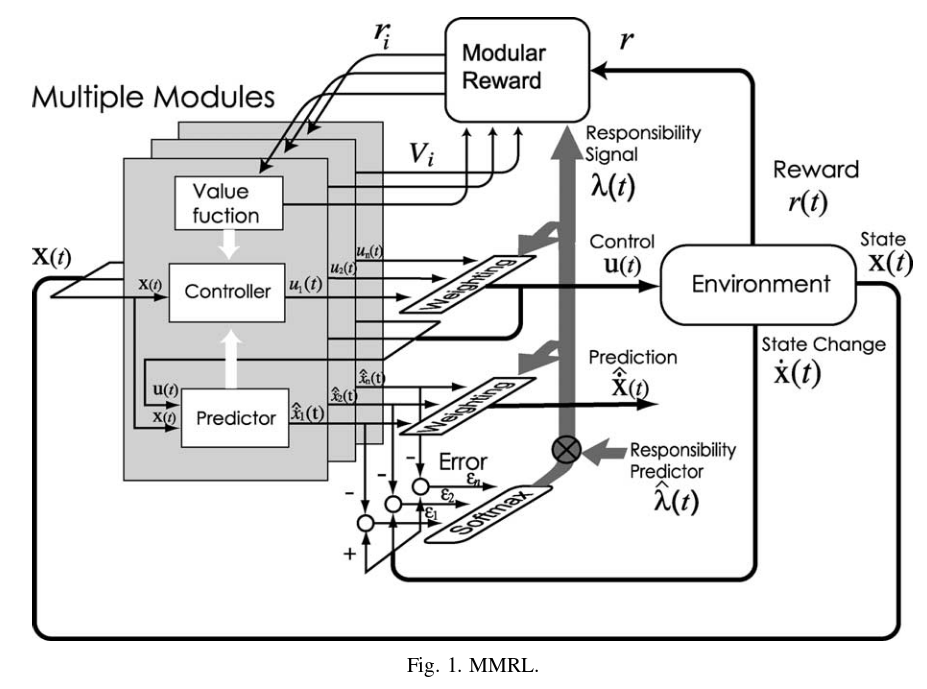
\includegraphics[width=0.8\columnwidth]{mrl.png}



MDP:
\begin{itemize}
  \item State: {\color{red}$S_1 \times S_2 \cdots \times S_M $}.
  \item Action: $A$.
  \item Transition: {\color{red}$P_1 \times P_2 \cdots \times P_M $}.
  \item Reward: {\color{red}$R_1 \times R_2 \cdots \times R_M $}.
\end{itemize}



Topics for Future Work
\begin{itemize}
  \item Credit assignment.
  \item Learning task hierarchies.
  \item Dynamic abstraction. 
  \item Integrating Deep Learning. 
\end{itemize}


\chapter{Evaluations and Applications}
\label{chp:eval}
\input{nips15/3-grid_world.tex}
\input{nips15/4-human}

\chapter{Conclusion}
\label{chp:conclude}
In this thesis, we followed an earlier work on modular inverse reinforcement
learning. We proposed a new modular inverse reinforcement
learning algorithm, and applied it to collected human subjects' data to analyze
their behavior.
The experimental results show that modular reinforcement learning can explain
human's navigation behavior. By our evaluation metrics, this method is better than other
baseline assumptions.

We have discussed in the literature review that modular approach is just one way to combine multiple
sub-MDPs. There are other assumptions that can be evaluated in the future work.
For example, scheduling between
different modules, with only one active at one time. This is close to the skill
switching method \cite{konidaris2009skill}. However, we adopt the
weighted sum approach because this is more reasonable for human behavior. When a
human tries to collect targets while avoiding obstacles, these two modules are
expected to be both active. A scheduling approach may yield frequent oscillation
between these two modules.

Static combination of modules throughout a task is another assumption that
should be removed in the future work. Parameters may be dynamic and different from
state to state.  However, with such an assumption we need to learn a mapping
from state to parameters. In this case, the curse of dimensionality still exists,
and inverse learning would be difficult.

So far, we only used the motion data of human subjects. There is also gaze data
collected but not used. Gazes are the points that human subjects are looking at
at a time step, which indicate humans' attention. This is actually a useful
information on how human combines different modules. When a human is paying
attention to a module, it is reasonable to assume that his action would be
affected mainly by this module.

In sum, we show in this thesis that modular reinforcement learning is a
promising explanation for human's navigation behavior. It is of interest to see
its analysis on different humans' behavior, and using the recovered parameters
for a learning agent to tackle similar tasks.


%%%%%%%%%%%%%%%%%%%%%%%%%%%%%%%%%%%%%%%%%%%%%%%%%%%%%%%%%%%%%%%%%%%%%%
% Appendix/Appendices                                                %
%%%%%%%%%%%%%%%%%%%%%%%%%%%%%%%%%%%%%%%%%%%%%%%%%%%%%%%%%%%%%%%%%%%%%%
%
% If you have only one appendix, use the command \appendix instead
% of \appendices.
%
\appendices
\index{Appendices@\emph{Appendices}}%

%%%%%%%%%%%%%%%%%%%%%%%%%%%%%%%%%%%%%%%%%%%%%%%%%%%%%%%%%%%%%%%%%%%%%%
% Generate the bibliography.					     %
%%%%%%%%%%%%%%%%%%%%%%%%%%%%%%%%%%%%%%%%%%%%%%%%%%%%%%%%%%%%%%%%%%%%%%
%								     %
% NOTE: For master's theses and reports, NOTHING is permitted to     %
%	come between the bibliography and the vita. The command      %
%	to generate the index (if used) MUST be moved to before      %
%	this section.						     %
%								     %
%\nocite{*}      % This command causes all items in the 		     %
                % bibliographic database to be added to 	     %
                % the bibliography, even if they are not 	     %
                % explicitly cited in the text. 		     %
		%						     %
\bibliographystyle{plain}  % Here the bibliography 		     %
\bibliography{diss,nips15/paper,RLLiterature/report}        % is inserted.			     %
\index{Bibliography@\emph{Bibliography}}%			     %
%%%%%%%%%%%%%%%%%%%%%%%%%%%%%%%%%%%%%%%%%%%%%%%%%%%%%%%%%%%%%%%%%%%%%%


%%%%%%%%%%%%%%%%%%%%%%%%%%%%%%%%%%%%%%%%%%%%%%%%%%%%%%%%%%%%%%%%%%%%%%
% Generate the index.						     %
%%%%%%%%%%%%%%%%%%%%%%%%%%%%%%%%%%%%%%%%%%%%%%%%%%%%%%%%%%%%%%%%%%%%%%
%								     %
% NOTE: For master's theses and reports, NOTHING is permitted to     %
%	come between the bibliography and the vita. This section     %
%	to generate the index (if used) MUST be moved to before      %
%	the bibliography section.				     %
%								     %
\printindex%    % Include the index here. Comment out this line      %
%		% with a percent sign if you do not want an index.   %
%%%%%%%%%%%%%%%%%%%%%%%%%%%%%%%%%%%%%%%%%%%%%%%%%%%%%%%%%%%%%%%%%%%%%%


%%%%%%%%%%%%%%%%%%%%%%%%%%%%%%%%%%%%%%%%%%%%%%%%%%%%%%%%%%%%%%%%%%%%%%
% Vita page.							     %
%%%%%%%%%%%%%%%%%%%%%%%%%%%%%%%%%%%%%%%%%%%%%%%%%%%%%%%%%%%%%%%%%%%%%%

\begin{vita}
Shun Zhang was born in Jinan, China in 1990. He was enrolled in the integrated
BS/MS program at University of Texas at Austin and finished both degrees in
summer, 2015. He is enrolled in the Ph.D. program in Computer Science and
Engineering in fall, 2015 at University of Michigan --- Ann Arbor.
\end{vita}

\end{document}
